\documentclass{imposter}
%\documentclass[landscape]{imposter}



%\usepackage{geometry}                		% See geometry.pdf to learn the layout options. There are lots.
%\geometry{landscape}                		% Activate for rotated page geometry
\usepackage[parfill]{parskip}    		% Activate to begin paragraphs with an empty line rather than an indent
%\usepackage{graphicx}				% Use pdf, png, jpg, or eps§ with pdflatex; use eps in DVI mode
								% TeX will automatically convert eps --> pdf in pdflatex		
								
								
\usepackage{wrapfig}								
\usepackage[font=scriptsize,labelfont=bf]{caption}
\usepackage[font=scriptsize]{subcaption}
\usepackage{float}
% \graphicspath{ {images/poster-eps/} }
\usepackage{amssymb}
\usepackage{amsmath}
\usepackage{bbm}

\usepackage{todonotes}

\graphicspath{ {../papers/halfdisk/images/} }
\graphicspath{ {images/} }

\newcommand{\sotodo}{\todo[color=green]}
\newcommand{\sotodoinline}{\todo[color=green,inline=true]}
\newcommand{\bstodo}{\todo[color=pink]}
\newcommand{\bstodoinline}{\todo[color=pink,inline=true]}



%SetFonts

%SetFonts

\usepackage{natbib}
\usepackage{url}
\bibliographystyle{abbrv}

\newcommand{\half}{\frac{1}{2}}
\newcommand{\R}{\mathbb{R}}
\newcommand{\C}{\mathbb{C}}
\newcommand{\Z}{\mathbb{Z}}
\newcommand{\N}{\mathbb{N}}
\newcommand{\No}{\mathbb{N}_0}
\newcommand{\Ylm}{Y^m_l}
\newcommand{\Ylmfull}{Y^m_l(\theta,\varphi)}
\newcommand{\Plm}{P^m_l}
\newcommand{\costheta}{\cos\theta}
\newcommand{\sintheta}{\sin\theta}
\newcommand{\cosphi}{\cos\varphi}
\newcommand{\sinphi}{\sin\varphi}
\newcommand{\eimphi}{e^{im\varphi}}
\newcommand{\alphalm}{\alpha^m_l}
\newcommand{\clm}{c^m_l}
\newcommand{\ctilde}{\tilde{c}^m_l}
\newcommand{\ctildemod}{\tilde{c}^{|m|}_l}
\newcommand{\chat}{\hat{c}^m_l}
\newcommand{\chatmod}{\hat{c}^{|m|}_l}
\newcommand{\ddx}{\frac{\mathrm{d}}{\mathrm{d}x}}
\newcommand{\dmdxm}{\frac{\mathrm{d}^m}{\mathrm{d}x^m}}

\newcommand{\Atilde}{\tilde{A}_{l,m}}
\newcommand{\Btilde}{\tilde{B}_{l,m}}
\newcommand{\Dtilde}{\tilde{D}_{l,m}}
\newcommand{\Etilde}{\tilde{E}_{l,m}}
\newcommand{\Ftilde}{\tilde{F}_{l,m}}
\newcommand{\Gtilde}{\tilde{G}_{l,m}}
\newcommand{\Alm}{A_{l,m}}
\newcommand{\Blm}{B_{l,m}}
\newcommand{\Dlm}{D_{l,m}}
\newcommand{\Elm}{E_{l,m}}
\newcommand{\Flm}{F_{l,m}}
\newcommand{\Glm}{G_{l,m}}

\newcommand{\xione}{\xi^{(1)}_{n, \lambda}}
\newcommand{\xitwo}{\xi^{(2)}_{n, \lambda}}
\newcommand{\xithree}{\xi^{(3)}_{n, \lambda}}
\newcommand{\xifour}{\xi^{(4)}_{n, \lambda}}

\newcommand{\bigP}{\mathbb{P}}
\newcommand{\Pl}{\mathbb{P}_l}
\newcommand{\gradP}{T\mathbb{P}}
\newcommand{\gradPl}{T\mathbb{P}_l}
\newcommand{\gradY}{\nabla Y}
\newcommand{\gradYlm}{\nabla Y^m_l}
\newcommand{\gradpY}{\nabla^\perp Y}
\newcommand{\gradpYlm}{\nabla^\perp Y^m_l}

\newcommand{\Dlt}{D^T_l}

\newcommand{\curlyy}{\bm{\mathcal{Y}}}
\newcommand{\blone}{\beta_{l, 1}}
\newcommand{\blzero}{\beta_{l, 0}}
\newcommand{\blmone}{\beta_{l, -1}}
\newcommand{\chivec}{\bm{\chi}_{1,m_s}}
\newcommand{\cgcoeff}{\mathcal{C}}

\newcommand{\alm}{a_{l,m}}
\newcommand{\blm}{b_{l,m}}
\newcommand{\dlm}{d_{l,m}}
\newcommand{\elm}{e_{l,m}}
\newcommand{\flm}{f_{l,m}}
\newcommand{\glm}{g_{l,m}}
\newcommand{\hlm}{h_{l,m}}
\newcommand{\jlm}{j_{l,m}}
\newcommand{\klm}{k_{l,m}}
\newcommand{\almperp}{a_{l,m}^\perp}
\newcommand{\blmperp}{b_{l,m}^\perp}
\newcommand{\dlmperp}{d_{l,m}^\perp}
\newcommand{\elmperp}{e_{l,m}^\perp}
\newcommand{\flmperp}{f_{l,m}^\perp}
\newcommand{\glmperp}{g_{l,m}^\perp}
\newcommand{\hlmperp}{h_{l,m}^\perp}
\newcommand{\jlmperp}{j_{l,m}^\perp}
\newcommand{\klmperp}{k_{l,m}^\perp}

\newcommand{\unitvec}{\hat{\bm{k}}}

\newcommand{\Pnk}{P_{n,k}}
\newcommand{\Pnkab}{P_{n,k}^{(a,b)}}
\newcommand{\Wab}{{W^{(a,b)}}}
\newcommand{\Pmjab}{P_{m,j}^{(a,b)}}
\newcommand{\alphaab}{\alpha^{(a,b)}}
\newcommand{\betaab}{\beta^{(a,b)}}
\newcommand{\bigPab}{\bigP^{(a,b)}}
\newcommand{\Dnt}{D^T_n}
\newcommand{\Wii}{W^{(1,1)}}
\newcommand{\Pii}{P^{(1,1)}}
\newcommand{\bigPii}{{\mathbb{P}^{(1,1)}}}
\newcommand{\Poo}{P^{(0,0)}}
\newcommand{\bigPoo}{{\mathbb{P}^{(0,0)}}}
\newcommand{\Poi}{P^{(0,1)}}
\newcommand{\Pio}{P^{(1,0)}}
\newcommand{\dx}{\frac{\partial}{\partial x}}
\newcommand{\dy}{\frac{\partial}{\partial y}}
\newcommand{\element}{\tau}
\newcommand{\refelement}{\hat{\tau}}
\newcommand{\FEset}{\mathcal{T}}
\newcommand{\bigW}{\mathbb{W}}
\newcommand{\bigWii}{{\mathbb{W}^{(1,1)}}}

\usepackage{amsthm}

\newtheorem{proposition}{Proposition}
\newtheorem{lemma}{Lemma} 
\newtheorem{theorem}{Theorem} 
\newtheorem{definition}{Definition}


\def\addtab#1={#1\;&=}

\def\meeq#1{\def\ccr{\\\addtab}
%\tabskip=\@centering
 \begin{align*}
 \addtab#1
 \end{align*}
  }  
  
  \def\leqaddtab#1\leq{#1\;&\leq}
  \def\mleeq#1{\def\ccr{\\\addtab}
%\tabskip=\@centering
 \begin{align*}
 \leqaddtab#1
 \end{align*}
  }  


\def\vc#1{\mbox{\boldmath$#1$\unboldmath}}

\def\vcsmall#1{\mbox{\boldmath$\scriptstyle #1$\unboldmath}}

\def\vczero{{\mathbf 0}}


%\def\beginlist{\begin{itemize}}
%
%\def\endlist{\end{itemize}}


\def\pr(#1){\left({#1}\right)}
\def\br[#1]{\left[{#1}\right]}
\def\fbr[#1]{\!\left[{#1}\right]}
\def\set#1{\left\{{#1}\right\}}
\def\ip<#1>{\left\langle{#1}\right\rangle}
\def\iip<#1>{\left\langle\!\langle{#1}\right\rangle\!\rangle}

\def\norm#1{\left\| #1 \right\|}

\def\abs#1{\left|{#1}\right|}
\def\fpr(#1){\!\pr({#1})}

\def\Re{{\rm Re}\,}
\def\Im{{\rm Im}\,}

\def\floor#1{\left\lfloor#1\right\rfloor}
\def\ceil#1{\left\lceil#1\right\rceil}


\def\mapengine#1,#2.{\mapfunction{#1}\ifx\void#2\else\mapengine #2.\fi }

\def\map[#1]{\mapengine #1,\void.}

\def\mapenginesep_#1#2,#3.{\mapfunction{#2}\ifx\void#3\else#1\mapengine #3.\fi }

\def\mapsep_#1[#2]{\mapenginesep_{#1}#2,\void.}


\def\vcbr[#1]{\pr(#1)}


\def\bvect[#1,#2]{
{
\def\dots{\cdots}
\def\mapfunction##1{\ | \  ##1}
	\sopmatrix{
		 \,#1\map[#2]\,
	}
}
}

\def\vect[#1]{
{\def\dots{\ldots}
	\vcbr[{#1}]
}}

\def\vectt[#1]{
{\def\dots{\ldots}
	\vect[{#1}]^{\top}
}}

\def\Vectt[#1]{
{
\def\mapfunction##1{##1 \cr} 
\def\dots{\vdots}
	\begin{pmatrix}
		\map[#1]
	\end{pmatrix}
}}



\def\thetaB{\mbox{\boldmath$\theta$}}
\def\zetaB{\mbox{\boldmath$\zeta$}}


\def\newterm#1{{\it #1}\index{#1}}


\def\TT{{\mathbb T}}
\def\C{{\mathbb C}}
\def\R{{\mathbb R}}
\def\II{{\mathbb I}}
\def\F{{\mathcal F}}
\def\E{{\rm e}}
\def\I{{\rm i}}
\def\D{{\rm d}}
\def\dx{\D x}
\def\dy{\D y}
\def\CC{{\cal C}}
\def\DD{{\cal D}}
\def\U{{\mathbb U}}
\def\A{{\cal A}}
\def\K{{\cal K}}
\def\DTU{{\cal D}_{{\rm T} \rightarrow {\rm U}}}
\def\LL{{\cal L}}
\def\B{{\cal B}}
\def\T{{\cal T}}
\def\W{{\cal W}}


\def\tF_#1{{\tt F}_{#1}}
\def\Fm{\tF_m}
\def\Fab{\tF_{\alpha,\beta}}
\def\FC{\T}
\def\FCpmz{\FC^{\pm {\rm z}}}
\def\FCz{\FC^{\rm z}}

\def\tFC_#1{{\tt T}_{#1}}
\def\FCn{\tFC_n}

\def\rmz{{\rm z}}

\def\chapref#1{Chapter~\ref{Chapter:#1}}
\def\secref#1{Section~\ref{Section:#1}}
\def\exref#1{Exercise~\ref{Exercise:#1}}
\def\lmref#1{Lemma~\ref{Lemma:#1}}
\def\propref#1{Proposition~\ref{Proposition:#1}}
\def\warnref#1{Warning~\ref{Warning:#1}}
\def\thref#1{Theorem~\ref{Theorem:#1}}
\def\defref#1{Definition~\ref{Definition:#1}}
\def\probref#1{Problem~\ref{Problem:#1}}
\def\corref#1{Corollary~\ref{Corollary:#1}}
\def\appref#1{Appendix~\ref{Appendix:#1}}

\def\sgn{{\rm sgn}\,}
\def\Ai{{\rm Ai}\,}
\def\Bi{{\rm Bi}\,}
\def\wind{{\rm wind}\,}
\def\erf{{\rm erf}\,}
\def\erfc{{\rm erfc}\,}
\def\qqquad{\qquad\quad}
\def\qqqquad{\qquad\qquad}


\def\spand{\hbox{ and }}
\def\spodd{\hbox{ odd}}
\def\speven{\hbox{ even}}
\def\qand{\quad\hbox{and}\quad}
\def\qqand{\qquad\hbox{and}\qquad}
\def\qfor{\quad\hbox{for}\quad}
\def\qqfor{\qquad\hbox{for}\qquad}
\def\qas{\quad\hbox{as}\quad}
\def\qqas{\qquad\hbox{as}\qquad}
\def\qor{\quad\hbox{or}\quad}
\def\qqor{\qquad\hbox{or}\qquad}
\def\qqwhere{\qquad\hbox{where}\qquad}



%%% Words

\def\naive{na\"\i ve\xspace}
\def\Jmap{Joukowsky map\xspace}
\def\Mobius{M\"obius\xspace}
\def\Holder{H\"older\xspace}
\def\Mathematica{{\sc Mathematica}\xspace}
\def\apriori{apriori\xspace}
\def\WHf{Weiner--Hopf factorization\xspace}
\def\WHfs{Weiner--Hopf factorizations\xspace}

\def\Jup{J_\uparrow^{-1}}
\def\Jdown{J_\downarrow^{-1}}
\def\Jin{J_+^{-1}}
\def\Jout{J_-^{-1}}



\def\bD{\D\!\!\!^-}




\def\questionequals{= \!\!\!\!\!\!{\scriptstyle ? \atop }\,\,\,}

\def\elll#1{\ell^{\lambda,#1}}
\def\elllp{\ell^{\lambda,p}}
\def\elllRp{\ell^{(\lambda,R),p}}


\def\elllRpz_#1{\ell_{#1{\rm z}}^{(\lambda,R),p}}


\def\sopmatrix#1{\begin{pmatrix}#1\end{pmatrix}}

\def\socases#1{\begin{cases} #1 \end{cases}}


\def\Problem#1#2\par{\begin{problem}\label{pb:#1} #2\end{problem}}
\def\Theorem#1#2\par{\begin{theorem}\label{th:#1} #2\end{theorem}}
\def\Conjecture#1#2\par{\begin{conjecture}\label{conj:#1} #2\end{conjecture}}
\def\Proposition#1#2\par{\begin{proposition}\label{prop:#1} #2\end{proposition}}
\def\Definition#1#2\par{\begin{definition}\label{def:#1} #2\end{definition}}
\def\Corollary#1#2\par{\begin{corollary}\label{cr:#1} #2\end{corollary}}
\def\Lemma#1#2\par{\begin{lemma}\label{lm:#1} #2\end{lemma}}
\def\Example#1#2\par{\begin{example}\label{ex:#1} #2\end{example}}
\def\Remark #1\par{\begin{remark*}#1\end{remark*}}


\def\Proof{\begin{proof}}
\def\mqed{\end{proof}}


\def\Figuretwow[#1,#2]#3#4\par{
\begin{figure}[tb]
\begin{center}{
\includegraphics[width=#3]{Figures/#1}\includegraphics[width=#3]{Figures/#2}}
\end{center}
\caption{#4}\label{fig:#1} 
\end{figure}
}


\usepackage{listings}

\title{Sparse Spectral Methods on Disk Slices}
\author{Ben Snowball (Supervisors: Sheehan Olver (Main), Colin Cotter)}
\department{Department of Mathematics, MPE CDT}
\institution{Imperial College London}

%% Primary university logo.
%\logo{imperial.eps}
% Secondary logos (not supported in all poster styles)
%\logoa{AMCG.eps}

%% Options to set colors of multiple poster features.
\titlecolor{named}{Blue}
\postercolor{named}{Blue}
%\pagecolor{green}

\posterstyle{mpecdtstyle}


% This sets up boxes to have nice rounded corners and somewhat thicker lines
% than the default.
\psset{linecolor=postercolor,linewidth=.2,cornersize=absolute,linearc=0.5,framesep=0.5}



\begin{document}
%\showgrid

% LHS

  \leftbox{96}{
        \section{Abstract}
        
In recent years, sparse spectral methods have been derived using hierarchies of classical orthogonal polynomials (OPs) on intervals, disks, and triangles (e.g. \cite{olver2018recurrence}). Here, we extend this methodology to a hierarchy of non-classical orthogonal polynomials on disk slices (e.g. a half disk), building on the observation that sparsity is guaranteed due to the boundary being defined by an algebraic curve, and that the entries of partial differential operators can be determined using formulae in terms of (non-classical) univariate OPs. 
 
    }
    
    
  \leftbox{81}{
      \section{Orthogonal polynomials on the half disk}

By using a similar process to \cite[p55--56]{dunkl2014orthogonal} we can construct 2D orthogonal polynomials on $\Omega$ from 1D orthogonal polynomials on the intervals \([0,1]\) and \([-1,1]\).

\begin{proposition}
Let \(w_1 : (\alpha,\beta) \: \to \R\), \(w_2 : (\gamma,\delta) \: \to \R\) be weight functions with \(\alpha,\beta,\gamma,\delta \in \R\),
Then, \(\forall n,k = 0,1,2,\dots\) let \(\{p_{n,k}\}\) be polynomials orthogonal with respect to the weight \(\rho(x)^{2k+1} w_1(x)\), and \(\{q_{n}\}\) be polynomials orthogonal with respect to the weight \(w_2(x)\). Then
$$
\Pnk(x,y) := p_{n-k,k}(x) \: \rho(x)^k \: q_k(\frac{y}{\rho(x)}) \qquad\hbox{for} \qquad 0 \le k \le n, \: n = 0,1,2,\dots
$$
are orthogonal polynomials with respect to the weight \(W(x,y) := w_1(x) \: w_2(\frac{y}{\rho(x)}) \) on $\Omega$. 
\end{proposition}

Taking $\Omega$ as the half disk, the weight $W^{(a,b)}(x,y)$ results from setting:
\begin{align}
\begin{cases}
(\alpha,\beta, \gamma,\delta) &:= (0.1, -1, 1) \\
\rho(x) &:= (1-x^2)^{\half} \\
w_1(x) &:= x^a \: (1-x^2)^b \\
w_2(x) &:= (1-x^2)^b = (1-x)^b \: (1+x)^b.
\end{cases}
\end{align}

The weight $w_2(x)$ corresponds to the weight for the Jacobi polynomials \(\{P_n^{(b, b)}\}\). The weight $w_1(x)$ is non-classical and we introduce the notation \(\{H_n^{(a, b)}\}\) for the orthonormal polynomials. Thus we arrive at a two parameter family of 2D OPs \(\{\Pnk\}\) given by, for \(0 \le k \le n, \: n = 0,1,2,\dots,\)
\begin{align}
 \Pnk^{(a,b)}(x,y) := H_{n-k}^{(a, b+k+\half)}(x) \: \rho(x)^k \: P_k^{(b,b)}(\frac{y}{\rho(x)}), \quad (x,y) \in \Omega, 
\end{align}
orthogonal on \(\Omega\) with respect to the weight $W^{(a,b)}(x,y)$.

    }
    
    \leftbox{37}{
    	\section{Jacobi matrices and building the OPs}
Define, for some $N \in \No$:
\begin{align}
\bigPab_n := \begin{bmatrix}
		P^{(a,b)}_{n,-n}(x,y) \\
		\vdots \\
		P^{(a,b)}_{n,n}(x,y)
	\end{bmatrix} \in \R^{n+1}, 
\quad \quad 
\bigPab := \begin{bmatrix}
		\bigPab_0 \\
		\bigPab_1 \\
		\vdots \\
		\bigPab_N
	\end{bmatrix}.
\end{align}

\begin{lemma}
The three-term recurrences that $\Pnk^{(a,b)}(x,y)$ satisfies lead to Jacobi operators that correspond to multiplication by $x$ and $y$. Set $J_x^{(a,b)}, J_y^{(a,b)} \in \R^{\half (N+1)(N+2) \times \half (N+1)(N+2)}$ as the Jacobi matrices corresponding to
\begin{align}
J_x^{(a,b)} \bigPab(x,y) = x \bigPab(x,y), \quad J_y^{(a,b)} \bigPab(x,y) = y \bigPab(x,y).
\end{align}
Then  \(J_x^{(a,b)}, J_y^{(a,b)}\) have similar sparse (block-tridiagonal) Banded-Block-Banded structures.
\end{lemma}
Combining each system in (4) we can write this as a block-tridiagonal system of equations. Applying a preconditioner matrix to the system \citep{dunkl2014orthogonal} (p78), we can expand the resulting lower-triangular system to obtain the recurrence:
    \begin{align}
\begin{cases}
\bigPab_{-1}(x,y) := 0, \quad \bigPab_{0}(x,y) := P^{(a,b)}_{0,0} \\
\bigPab_{n+1}(x,y) = -\Dnt (B_n-G_n(x,y)) \bigPab_n(x,y) - \Dnt C_n  \,\bigPab_{n-1}(x,y).
\end{cases}
\end{align}
where the matrix coefficients $\Dnt, B_n, C_n, G_n(x,y)$ can be explicitly found.
    }
	
    
    \rightbox{96}{
    	\section{Sparse partial differential operators}

For general \(a,b\) and general functions \(f(x,y) = \bigPab(x,y)^\top \mathbf{f}\), there exist sparse operators \(D_x^{(a,b)}, \: D_y^{(a,b)}, \: W_x^{(a,b)}, \: W_y^{(a,b)}\) such that (as seen in the DLMF \cite{DLMFDerivatives} for other OP families):
\begin{align*}
\dx[f(x,y)] &= \bigP^{(a+1,b+1)}(x,y)^T \: D_x^{(a,b)} \: \mathbf{f}, \\
\dy[f(x,y)] &= \bigP^{(a,b+1)}(x,y)^T \: D_y^{(a,b)} \: \mathbf{f}, \\
\dx[\Wab(x,y) \: f(x,y)] &= W^{(a-1,b-1)}(x,y) \: \bigP^{(a-1,b-1)}(x,y)^T \: W_x^{(a,b)} \: \mathbf{f}, \\
\dy[\Wab(x,y) \: f(x,y)] &= W^{(a,b-1)}(x,y) \: \bigP^{(a,b-1)}(x,y)^T \: W_y^{(a,b)} \: \mathbf{f}.
\end{align*}
Further, we note that there exist Banded-Block-Banded matrix operators $T^{(1,0)\to(0,0)}\), \(T^{(0,1)\to(1,1)}$ such that:
\begin{align*}
x \bigP^{(1,0)}(x,y) &= \Big(T^{(1,0)\to(0,0)} \Big)^T \: \bigP^{(0,0)}(x,y) \\
\bigP^{(0,1)}(x,y) &= \Big(T^{(0,1)\to(1,1)} \Big)^T \: \bigP^{(1,1)}(x,y)
\end{align*}
\begin{align}
    \implies \Delta^{(1,1)} := D_x^{(0,0)} \: W_x^{(1,1)} + T^{(0,1)\to(1,1)} \: D_y^{(0,0)} \: T^{(1,0)\to(0,0)} \: W_y^{(1,1)},
\end{align}

\begin{wrapfigure}{R}{0.7\textwidth}
        \center 
   \begin{subfigure}[t]{0.35\textwidth}
         \centering
        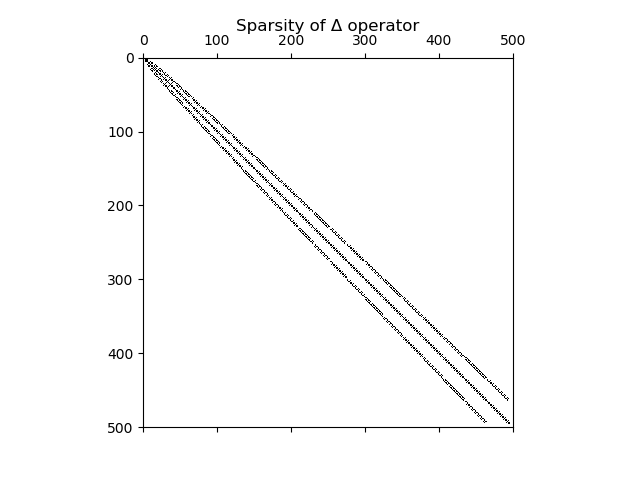
\includegraphics[scale=1.0]{sparsityoflaplacian}
        \label{fig:sparsity}
    \end{subfigure}
   \begin{subfigure}[t]{0.3\textwidth}
         \centering
        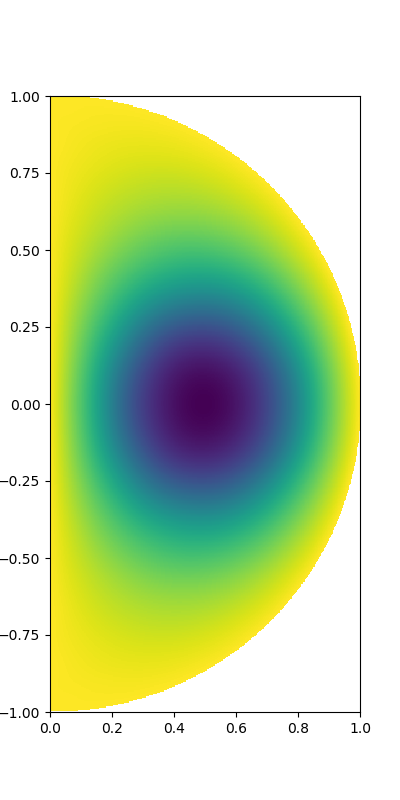
\includegraphics[scale=0.6]{solution}
        \label{fig:solution}
    \end{subfigure}
    \begin{subfigure}[t]{0.3\textwidth}
                \center
        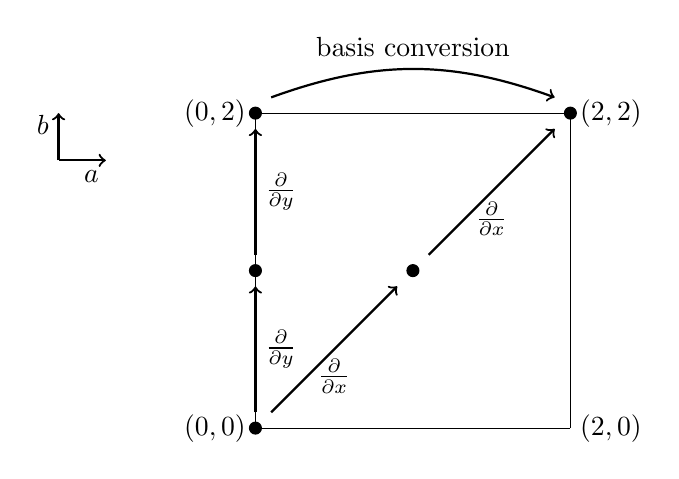
\begin{tikzpicture} 
        % Box/square (4x4)
        \draw[black,solid,ultra thin] (0,0)--(0,4);
        \draw[black,solid,ultra thin] (0,0)--(4,0);
        \draw[black,solid,ultra thin] (4,0)--(4,4);
        \draw[black,solid,ultra thin] (0,4)--(4,4);
        % Dots
        \draw[black,fill=black] (0,0) circle (.5ex);
        \draw[black,fill=black] (2,2) circle (.5ex);
        \draw[black,fill=black] (4,4) circle (.5ex);
        \draw[black,fill=black] (0,2) circle (.5ex);
        \draw[black,fill=black] (0,4) circle (.5ex);
        % Arrows
        \draw[black,thick,->] (0.2,0.2)--(1.8,1.8);
        \draw[black,thick,->] (2.2,2.2)--(3.8,3.8);
        \draw[black,thick,->] (0,0.2)--(0,1.8);
        \draw[black,thick,->] (0,2.2)--(0,3.8);
        \draw [black,thick,->] (0.2,4.2) to [out=20,in=160] (3.8,4.2);
        % Node (parameter) labels
        \draw[] (0,0) node[anchor=east] {$(0,0)$};
        \draw[] (0,4) node[anchor=east] {$(0,2)$};
        \draw[] (4,0) node[anchor=west] {$(2,0)$};
        \draw[] (4,4) node[anchor=west] {$(2,2)$};
        % Arrow labels
        \draw[] (1,1) node[anchor=north] {$\tfrac{\partial}{\partial x}$};
        \draw[] (3,3) node[anchor=north] {$\tfrac{\partial}{\partial x}$};
        \draw[] (0,1) node[anchor=west] {$\tfrac{\partial}{\partial y}$};
        \draw[] (0,3) node[anchor=west] {$\tfrac{\partial}{\partial y}$};
        % The key and headings
        \draw[black,thick,->] (-2.5,3.4)--(-2.5,4);
        \draw[black,thick,->] (-2.5,3.4)--(-1.9,3.4);
        \draw[] (-2.3,3.2) node[anchor=west] {$a$};
        \draw[] (-2.7,3.6) node[anchor=south] {$b$};
        \draw[] (2,4.6) node[anchor=south] {basis conversion};
        \end{tikzpicture} 
	\label{fig:Laplace}
   \end{subfigure}
    \centering
    \captionsetup{width=.7\linewidth}
    \caption{Left: A "spy" plot of the $\Delta$ operator for $\Wii(x,y) \: \bigPii(x,y) \to \bigPii(x,y)$ showing its sparsity. Right: The computed solution to $\Delta u = f$ with zero boundary conditions with $f(x,y) = 1 + \text{erf}(5(1 ? 10((x ? 0.5)^2 + y^2)))$. Bottom: Diagram illustrating how the parameters change under partial differentiation. }
\end{wrapfigure}

where $\Delta^{(1,1)}$ is the matrix operator for the Laplacian, that will take us from coefficients for expansion in the weighted space $\Wii(x,y) \: \bigPii(x,y)$ to coefficients in the non-weighted space $\bigPii(x,y)$. This operator will have Banded-Block-Banded structure, and hence sparse. Note that this construction ensures imposition of Dirichlet zero boundary conditions.

The sparsity of the these operators can be shown using a simply integration by parts argument, again showing that the sparsity for differential operators is not dependent on the domain.
 
    }
    
     \rightbox{30.5}{
      \section{Summary and Future Work}
      
\begin{itemize}
  \item We have detailed a method for obtaining families of 2D OPs on certain domains. Using the three-term recurrence relationships the OPs have, we can calculate sparse operator matrices for multiplication by $x, y$ and in turn sparse differential operators, allowing us to solve PDEs on the half disk.
  \item The same (or similar) relations hold for other suitable domains (namely, disk slices). 
  \item This 2D half disk framework can be extended for a family of OPs on the hemisphere, with sparse relations.
   \item To solve PDEs on spherical triangles (as is our ultimate goal) will require further ideas.
\end{itemize}
  
    }
    
%Also do graphics.
    \rightbox{11}{
        {\footnotesize\bibliography{../papers/halfdisk/halfdisk-bib}}
        
    }


\end{document}
